\chapter{Consistency through different transcriptomics studies with RNA-Seq}
\label{ch:Transcriptomics}
%\setlength{\epigraphwidth}{0.45\textwidth}
%\setlength{\epigraphrule}{0.1pt}
%\epigraph{Quantifier: c'est convenir, puis mesurer.}{\cite{Desrosieres}}


I started this project in January 2013. At that time, there was no
literature comparing normal human transcriptome tissues across different datasets.

\section{Introduction}

\begin{itemize}
    \item Difficulty of sampling of normal conditions for human, particularly
        for the solid tissues. (could be very useful in case of cancer for
        example)
    \item Lots of transcriptomics data in the repository of EBI. Can we use
        this as a base for reference? + Explosion of atlases publications
    \item previous point not new, but recently multiplications of studies on
        normal human studies based on \Rnaseq
    \item Indeed, in the past people tried with microarray data but didn't work
        \TK{find sources}
    \item When I started this study, there wasn't any publication on this matter
        yet, but \Rnaseq was considered as quantitative (when microarrays were
        considered semi-quantitative at best).
    \item nobody did published on my specific subject yet, but since then things changed
    \item first paper from MACQ/SEC III
    \item increasing number of papers that been published on the subject
    \item I will discuss the different part of the papers that are relevant
        with additions on what my study confirms/refutes or expands them.
\end{itemize}

Progress in Science is based on different elements. In natural sciences, notably
Biology, repeated observations are one of the earliest ones. Then quantifications
when possible (+ definitions give you characterisation). (They could be inferred or
been used as a start for a hypothesis and then there are predictions and
experiments). When many observations and measurements, common step: try to create
a reference. People tried with microarrays technologies but there were too many
biases and too different microarrays to work with. However, it would be very nice
to have a reference as it is hard to have a normal controls in studies. Hence, we
have seen a common trend of Atlases publications and even more when \Rnaseq\ started
to be used more commonly. (Explosion of the Atlases).

While current high-throughput gene expression studies are mainly about
differential gene expression between (notably diseased and treated) conditions,
healthy controls are not always enough or even available. Even more so, when the
study subject is human. Indeed, it rather apprehensible that sampling solid
tissues on a healthy human is not (and should not be) usual or common.

Although, many atlases have been released to help on this issue,
there is still not any direct method that would allow you more than check the
presence (or lack of detection) of specific genes in a given condition.

With the increasing number of studies of normal tissues with overlapping conditions
\cref{fig:VennStudiesT}, we are investigating the consistency of gene-tissue
associations on
one side but moreover we would like to assess the expression levels across the
datasets in the aim of integrating all the available data in a gene expression
baseline reference.

When I started this project there was not any study, comprehensive or not, that
was investigating in-depth the consistency of transcriptome expression measurements
for one condition across studies.

As previously stated in the introduction, while I started this project,
there wasn't any study that was investigating in-depth the reproducibility of
transcriptomics.

However, in August 2014 a paper comparing different preparation methods,
sequencing technologies operated in different laboratories
on samples from the same biological source concludes that while absolute
measurements are not consistent, the relative expression is highly consistent
(95\% Pearson correlation?)

The main question when I started this project was to appraise how much consistent
(robust) is the \Rnaseq technology to quantify the gene expression. While it
is comparable to microarrays for differential gene expression analysis study
\TK{add reference},
\Rnaseq\ plus: detect new things - minus: sampling problems (stuff might be there
but won't be ``fished''.

%%%%%%%%%

When I started this work in 2013, there were only three complying
datasets at that time. Fortunately, I was later
able to incorporate two other datasets to my study. One of them is the \Gtex\
pilot (version 1.4) data and the other one is the Uhlén et al.\ dataset (first
published as \citet{Uhlen2014} and then extended for the \citet{Uhlen2015} publication).
The number of provided samples and covered tissues for these two datasets
is far greater than the other ones. These \dataset{\Gtex} and \dataset{Uhlén}
datasets are indeed presenting a greater set of common tissues. Moreover,
the more recent and similar technology used (either for the libraries preparation,
the sequencer or the paired-end protocols) and the studies design that includes
biological replicates for every tissue had motivated a more focused comparison
based only on these two datasets.

While I downloaded and entirely processed four of the transcriptomic datasets
myself, it was not the case for the \Gtex\ dataset. Since this
data is involved in many project within the \EBI\ and due to its huge amount of
data, it was agreed that this would be processed centrally by one person and then
redistributed to all the other interested parties. Dr Nuno Fonseca had this
tremendous task and provided me with quantification data,
both for each sample separately and then for each tissue (all relevant samples
pooled together).

For the sake of consistency, that led me to reprocess all the other four datasets
to comply with the reference used for the \Gtex\ samples. The silver lining
was that they were built with the new reference of the
Human genome GRCH 38 (ENSEMBL v. 76).

\begin{figure}%[!htbp]
    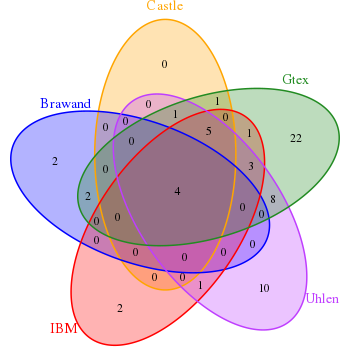
\includegraphics[scale=0.6]{transcriptomics/VennStudiesT}\centering
    \caption[Distribution of unique and shared tissues between the
    transcriptomic datasets]
    {\label{fig:VennStudiesT}\textbf{Distribution of unique and shared tissues
    between the transcriptomic datasets.} The 5 datasets share 4
    common tissues: \tissue{Heart}, \tissue{Kidney}, \tissue{Liver} and
    \tissue{Testis}. The biggest overlap of tissues (23) is between Uhlén et \Gtex.
    These two sets of tissues are the focus of the current study.}
\end{figure}

\Cref{fig:VennStudiesT} presents the five datasets overlapping tissues. We notice
that they all share at least four tissues: \tissue{Heart}, \tissue{Kidney},
\tissue{Liver} and \tissue{Testis}.

We also observe the great number of shared tissues between the two most recent
datasets: \dataset{Uhlen} and \dataset{GTEx}. Indeed, they share together twenty-three
tissues: \tissue{Adipose}, \tissue{Adrenal}, \tissue{Bladder},
\tissue{Cerebral cortex}, \tissue{Colon}, \tissue{Oesophagus},
\tissue{Fallopian tube}, \tissue{Heart}, \tissue{Kidney}, \tissue{Liver},
\tissue{Lung}, \tissue{Ovary}, \tissue{Pancreas}, \tissue{Prostate},
\tissue{Salivary gland}, \tissue{Skeletal muscle}, \tissue{Skin},
\tissue{Small intestine}, \tissue{Spleen}, \tissue{Stomach}, \tissue{Testis},
\tissue{Thyroid} and \tissue{Uterus}.

As we can see in the \cref{tab:Trans5DF}, many of the transcriptomic datasets I
use have been produced through
polyA-selected library protocols, notably the \dataset{Uhlén} dataset which is
used in both study parts.
To avoid as many artefacts as possible, I
focus my study on the \mRNAs\ pool: most of the analyses are excluding
any gene that the biotype is not annotated as \emph{protein coding}.

\begin{comment}
\begin{sidewaystable}
    \centering
    \caption{\label{tab:Trans5DF}Technical description of the 5 transcriptomic
    dataset (\Rnaseq)
     used for this study}
\begin{tabular}{@{}cccccccccc@{}}
\toprule
\multicolumn{1}{c|}
    {\multirow{2}{*}{ArrayExpress ID}} &
     \multicolumn{1}{c|}{\multirow{2}{*}{Data ID}} &
     \multicolumn{2}{c|}{\begin{tabular}[c]{@{}c@{}}Library\\Preparation\end{tabular}} &
     \multicolumn{2}{c|}{Sequencing} &
     \multicolumn{2}{c|}{Replicates} &
     \multicolumn{1}{c|}{\multirow{2}{*}{\begin{tabular}[c]{@{}c@{}}Tissue\\
             Number\end{tabular}}} &
     \multirow{2}{*}{\begin{tabular}[c]{@{}c@{}}Multi-sampling\\ from the \\ same individual\end{tabular}} \\
     \cmidrule(lr){3-8}
     \multicolumn{1}{c|}{} & \multicolumn{1}{c|}{} &
     \multicolumn{1}{c|}{\begin{tabular}[c]{@{}c@{}}Whole\\ RNA\end{tabular}} &
     \multicolumn{1}{c|}{\begin{tabular}[c]{@{}c@{}}PolyA\\ selected\end{tabular}} &
     \multicolumn{1}{c|}{\begin{tabular}[c]{@{}c@{}}Single\\ end\end{tabular}} &
     \multicolumn{1}{c|}{\begin{tabular}[c]{@{}c@{}}Paired\\ end\end{tabular}} &
     \multicolumn{1}{c|}{Biological} & \multicolumn{1}{c|}{Technical} &
     \multicolumn{1}{c|}{} &  \\
\midrule
E-MTAB-305 & Castle & Y &  & Y &  &  &  & 11 &  \\
E-GEOD-30352 & Brawand &  & Y & Y &  & Y &  & 8 &  \\
E-MTAB-513 & IBM &  & Y & Y & Y &  & (Y) & 16 &  \\
E-MTAB-2836 & Uhlén &  & Y &  & Y & Y & Y & 32 &  \\
E-MTAB-2919 & Gtex  & Y &  &  & Y & Y &  & 54 & Y \\
\bottomrule
\end{tabular}
\end{sidewaystable}


\section{Clustering analysis}

As we know the tissue type for each sample, we could debate that a supervised
analysis can be more informative. However, it would involve proper corrections
for batch effects and other technical biases for each dataset.
This is challenging as that often requires more knowledge than the available one
through the repositories. It is also unwise to rely solely on the normalised data
provided by the original authors as bias corrections (when possible)
in \Rnaseq\ will vary in function of the following downstream analyses.

To assess the consistency of \Rnaseq\ quantification across the different
datasets, I chose a widely used and unsupervised method for gene
expression studies: a cluster analysis.

This method uncovers possible hidden structures within the data, therefore,
it is well designed for this exploratory study.
I can then confirm if samples are more alike either due to their
biological or their study origins. We expect in general biology to be a better
predictor. Yet, a technical predictor can not be excluded straightforwardly
as most transcripts (in particular \mRNAs) are expressed in many tissues
and two random tissues share about 60 to 90\%  of their pool of \mRNAs\
\citep{ramskoldan:2009}, \citep{UhlenGastro}.

There are many available algorithms for clustering analysis.
Each one based on different notions and approaches.
I chose a \emph{hierarchical} clustering (or \emph{connectivity-based} clustering).

This sort of clustering is broadly used in gene expression studies as it is
embryologically\footnote{Or evolutionary, when different species are compared}
pertinent as we know that the whole organism is developed from
an original single cell. The data is portioned in an extensive hierarchy:
each cluster merges with another at a certain distance.
In practice, each sample starts in its own cluster and then
by iteration, each cluster is merged with nearest one. The method has
two parameters: the linkage and the distance.

The linkage specifies which part of each cluster is used as reference
for computing the distance between the clusters. There are many methods and after
trying many of them, I picked arbitrary the one that was accurately dividing
the samples by tissues for every and each of the different datasets.

The distance measures the dissimilarity between two samples and one common
approach is to calculate the subtraction result of
the correlation coefficient from $1$ (as smaller is the difference, greater is
the similarity shared between the two samples).

Correlation coefficients are a measure of the statistic dependence between two
variables (here the samples) and always ranges within $[-1,1]$. They pairwise
compare observations between the two variable. Most implementation methods
will manage an unbalanced number of observations by excluding the incomplete pairs.
To ease the interpretation I preferred to filter the data \latin{a priori}
myself; I only kept expression values effectively observed in all the datasets
(\cref{sec:TransExpressedOrNot}).

There are several methods available to compute the correlation coefficient; the
most famous and used are the Pearson and the Spearman correlation coefficients.
I tried both.

The Spearman correlation is more robust than the Pearson
correlation. However, it only assesses the monotonic dependence between samples.
The Pearson correlation also assesses the linear dependence between them.
Now, this study is part of a broader scheme that aims to provide \latin{in fine}
a reference for the Human transcriptome. In this context, Pearson correlation
coefficients give a better estimation on the practical feasibility.

\section{Expressed or not expressed}
\label{sec:TransExpressedOrNot}
While it can seem as a trivial concept and might be overlook, whether a specific
molecule is expressed --- or not --- in a given condition, can actually have
an extensive impact on the results of the analyses, particularly when we compare
different studies.

For example, the Pearson correlation coefficient is very
sensitive to outliers and null values. If for both samples, a vast number of
null values are recorded, this will lead to a greater similarity.
Hence, it is important that the data used for the analysis is meaningful in
its whole, i.e.\ a null value has still to be an observation and translates
a lack of expression (and not a lack of observation).

\begin{figure}[!htbp]
  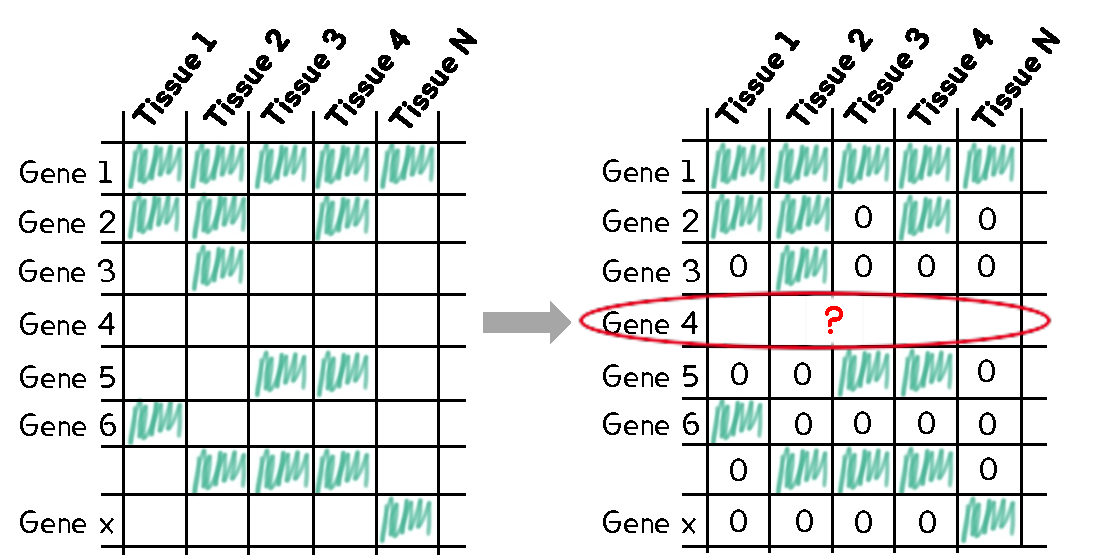
\includegraphics[scale=0.8]{integration/expressedNotExp.pdf}\centering
      \caption[Expressed or not: several cases illustrated]
      {\label{fig:DefineExpression}\textbf{Expressed or not: several cases
      illustrated.}\smallbreak{}Genes as \emph{gene 1} are unequivocal: they have been
      detected in all the different tissues. Genes that have been quantified in
      \emph{some} of the conditions are, in principal, detectable with the
      protocol of sampling and quantification used for the assay.
      For these genes, when no signal is collected, I assume this is a true $0$.
      The genes without any quantification
      in any tissue, e.g.\ gene 4, are discarded from the remaining analysis as
      I can't state
      either there are truly absent from the biological sample or it has to due
      to the protocol at use; they are \emph{undefined}.}
\end{figure}

\subsection{The undefined}\KOMAoptions{parskip=false}
\label{subsec:IntegrationExpressedOrNot-undefined}
If a transcript is never found in any of the samples of a dataset,
then I considered that we can not determine if the transcript was
either truly not expressed or, for any reason, was not captured while the library
preparation or the identification/quantification steps. Hence, those are
excluded from the analyses as I can not resolve precisely if this is a
technical artefact or a biological truth. This case is illustrate by the row
circled in red in~\cref{fig:DefineExpression}.

\subsection{Expression in a dataset}
\label{subsec:IntegrationExpressedOrNot--expDataset}
By contrast, if a transcript is expressed in any sample of the dataset,
then, whenever no expression was recorded in the other
samples, I consider that the expression of the considered macromolecule is truly
null for those samples.

\subsection{Expression within a sample}\KOMAoptions{parskip=half*}\label{subsec:exprTrans}
It is a little trickier as we have to account for technical noise,
but we can also expect ``translational noise'' \citep{rnaseq-2009},
\citep{lowNoiseLimit}.
While we can empirically evaluate it for each dataset \citep{ramskoldan:2009},
there is a widespread (arbitrary) threshold used in the literature:
1 \gls{FPKM} (or \gls{RPKM}).
I have used this threshold to run (at least once) all the analyses since
many datasets are enriched for \mRNAs. Moreover, the \Cref{ch:Integration}
focus is the comparison of proteomic and
transcriptomic data. In fact,~\citet{Hebenstreit:2011} showed in
their study \paper{\citetitle{Hebenstreit:2011}},
that to be translated into a protein, a \mRNA\ should
present an expression at least equals to 1 \gls{RPKM}.

It is worth mentioning that parts of the analyses have also been done without
any threshold or with a threshold of $5$ \glspl{FPKM}.

\subsection{Limitation of the study}
While I have compared the list of undefined, expressed and unexpressed \mRNAs\
through the five datasets, the bulk of the analysis has been done on the common
\mRNAs.

In other words, if a \mRNA\ is not expressed in at least one sample in \emph{each}
dataset used for the study, it will be excluded from the main part of the
analysis workflow.

\end{comment}

\section{Results}\label{sec:Trans_Results}
\section{Methods}
\subsection{A consistent \Rnaseq\ workflow}
%The Pearson product-moment correlation coefficient (often shortened as
%Pearson correlation coefficient or even as correlation coefficient) is a

%
\subsubsection{The expectation}
$E[X]=x_1p_1 + x_2p_2+ \cdots +x_kp_k$

\begin{itemize}
\item $E$ is the expectation
\item $X$ is a random variable
\item $x_1$,$x_2$,\ldots,$x_k$ are possible value of $X$
\end{itemize}




\section{Consistency of processing methodology}\label{sec:Trans_consistentMethodo}

    \subsection{Reuse of processed data issues}\label{subsec:Trans_reuseOfData}

    \subsection{Genome build and annotation impact}\label{subsec:Trans_AnnotImpact}

RNA-seq is consistent across datasets; samples are more likely to cluster by
biological origins than by studies. (Figure 2)
While Pearson correlations are higher, without any a priori Spearman correlations
allow a better separation of the different tissues in distinct clusters across
datasets.

Many genes have a consistent profile of expression levels through the different
datasets.
To help EBI Expression Atlas has developed a feature that allows the visualisation
of the expression of a gene (or protein) across the different dataset that it
integrates. (Figure 3)

Reuse of data allows the assessment of the biological quality of a sample.
While RNA-seq workflows integrate numerous quality checks for their different steps,
it is not always easy to appraise the original quality of the samples. Comparing
similar conditions from different sources allow some high level biological check.
Indeed, we noticed that some tissues have a more unique profile in specific
datasets.

Overall gene expressions for protein coding genes across different tissues
correlated highly between datasets. (See part 3. Integration of Transcriptomics
and Proteomics studies – Figure 15)



    \subsection{Reproducibility of expression profile at tissue level}\label{subsec:Trans_ReproExpresTissue}

        \subsubsection{Correlation}\label{subsubsec:Trans_Tissue_Corr}
        \subsubsection{Clustering}\label{subsubsec:Trans_Tissue_cluster}

    \subsection{Reproducibility of expression profile at gene level}\label{subsec:Trans_ReproExpresGene}

    \subsection{Tissue specific,housekeeping genes and other categories}\label{subsec:Trans_TissueSpeAndHK}

    \subsection{Curated sets}\label{subsec:Trans_curatedSets}

\section{Discussion}\label{sec:Trans_discussion}



\begin{comment}
  \begin{figure}%[!htbp]
      \includegraphics%[scale=0.6]%
      {transcriptomics/}\centering
      \caption[]
      {\label{fig:}\textbf{}}
  \end{figure}
\end{comment}
